\documentclass[12pt]{article}

\usepackage[utf8]{inputenc}
\usepackage[T1]{fontenc}
\usepackage{geometry}
\usepackage{graphicx} %figures
\usepackage{subfig} %subfigures
\usepackage{gensymb} %degree sign
\usepackage{amsmath} %math stuff
\usepackage{bm} %bold stuff
\usepackage[]{algorithm2e} %algorithms
\geometry{a4paper}

\title{\textbf{Part 4: MCMC and Bayesian Modeling Part I}}

\begin{document}
\date{January 4, 2021}
\maketitle

I would not presume to know very much about Bayesian modeling, but I have been learning more and this post should provide a good foundation for further exploration. First I will provide some background to the types of models we will be working with then some methods (Gibbs Sampling and Hamiltonian-Monte Carlo Sampling) for solving said models.

\vspace{5mm}

The cornerstone of Bayesian Modeling is \emph{Bayes Rule}:

\begin{equation}
Pr(\theta | x) = \dfrac{Pr(\theta) Pr(x | \theta)}{Pr(x)} \propto \pi(\theta) p(x | \theta)
\end{equation}

Normally the next few pages would be filled with explanations about marginalization and solving for moments, means, and modes for a million different distributions but I will keep it simple. If we want to fit a statistical model with parameters $\theta$ with data $x$ we want to maximize $Pr(\theta | x)$, which the the probability of the parameters given data, also called the \emph{posterior} distribution. So in a simple linear model we want to maximize the probability that the data $x$ fits the model given slope and intercept $\theta = \{\alpha,\beta\}$.

\vspace{5mm}

This posterior proportional to $\pi(\theta)$, the prior (do I think the slope will be big or small for example) multiplied by $p(x | \theta)$, the likelihood (how well the data fits to the slope for example). This is how Bayesian statistics works: we weight how well the data fits the model with our prior belief about the model. This may introduce subjectivity to the model (it does) but it also allows us to regularize the model. You may remember "regularization" from the RBF discussion, but basically a more regularized model will make fewer extreme predictions. We can constrain our model parameters $\theta$ to be more \emph{skeptical} of the data $x$. 

\begin{figure}[h]
\centering
\subfloat[][Raw Data]{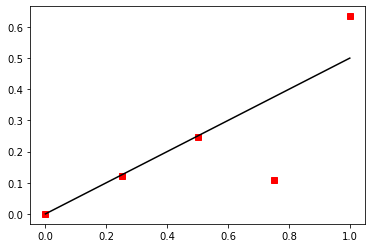
\includegraphics[width=0.3\textwidth]{Post_4_bayes1}}
\hspace{1cm}
\subfloat[][Prior of $\beta$]{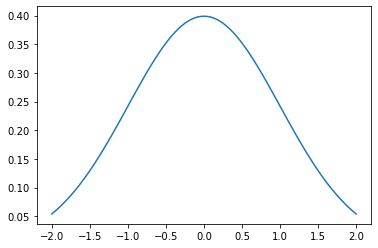
\includegraphics[width=0.3\textwidth]{Post_4_bayes2}}

\subfloat[][Likelihood]{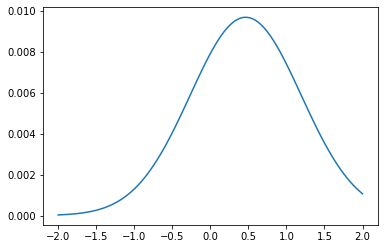
\includegraphics[width=0.3\textwidth]{Post_4_bayes3}}
\hspace{1cm}
\subfloat[][Posterior]{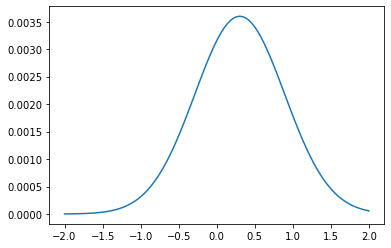
\includegraphics[width=0.3\textwidth]{Post_4_bayes4}}
\caption{Bayesian Model for $Y = \beta X + \epsilon$ where $\epsilon \sim N(0,Y/2)$}
\end{figure}

\vspace{5mm}

Here we model a process $Y = \beta X + \epsilon$ where $\epsilon \sim N(0,Y/2)$ using a normal prior for the slope $\beta$ of $\beta \sim N(0,1)$ so that the optimal $\beta$ is regularized around zero. We multiply that by a likelihood model $\beta X - Y \sim N(0,1)$, which is to say we expect the error in the linear model to be around zero with some deviance of one. Therefore, by Equation (1) the posterior is:

\begin{equation}
\beta | x \sim N(\beta,0,1) \: \Pi_i^N N(\beta X_i - Y_i,0,1)
\end{equation}

\vspace{5mm}

Notice that the posterior is just a jumble of stacked distributions asking the question "\emph{what's up with this $\beta$?}". From Figure 1 (b) and (c) we see that the prior wants to say zero, and the likelihood wants to say $0.5$. For more complex problems the prior will help to regularize the likelihood a bit more obviously than here.

\section{Gibbs Sampling}

It's easy enough to sample from a posterior in a single dimension and visually inspect the maximum (also called \emph{maximum a posterior} MAP estimate). However in many dimensions we need other methods to "sample" distributions. These sampling methods then give us estimates of the best parameters that explain the data/integrate in our priors.

\vspace{5mm}

The Gibbs Sample is one such method. The algorithm is simple:

\begin{algorithm}[H]
 \KwData{$Pr(\theta_i | \theta_{-i},x)$ Marginal Posterior Equations}
 \KwResult{$\Theta \sim Pr(\theta | x)$ Posterior Sample}
\For{$k = 1:K$ Samples}{
\For{$i = 1:d$ Parameters}{
Marginalize $\theta \sim Pr(\theta_i | \theta_{-i}, x)$\;
Append $\theta$ to $\Theta$\;}}
 \caption{Gibbs Sample}
\end{algorithm}

\vspace{5mm}

All one needs to know is the marginal equations of the posterior $Pr(\theta_i | \theta_{-i},x)$ for parameter $\theta_i$ with all other parameters $\theta_{-i}$ integrated out. This is easy enough with, say, independent distributions such as two normal distributions:

\begin{align*}
Pr(\theta_0,\theta_1 | \mu_0 = 1, \mu_1 = 2) = N(\theta_0 | \mu_0, \sigma)N(\theta_1 | \mu_1, \sigma)
\end{align*}

\begin{figure}[h]
\centering
\subfloat[][Sample]{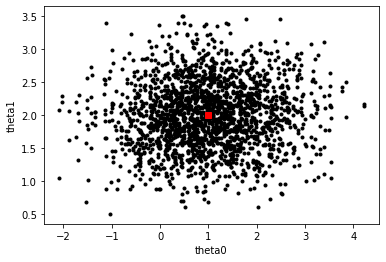
\includegraphics[width=0.3\textwidth]{Post_4_normal1}}
\subfloat[][Distributions]{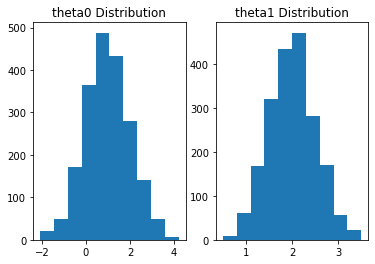
\includegraphics[width=0.3\textwidth]{Post_4_normal2}}
\caption{Gibbs Sample of Two Independent Normals $\mu_0 = 1$ and $\mu_1 = 2$}
\end{figure}

\vspace{5mm}

The same can be done with two dependent distributions; a Beta and Binomial distribution. In this example, it is desired to model a posterior $Pr(x,y)$ with a complicated distribution. The posterior looks like this (I've stolen this from IEOR E4703: Monte Carlo Simulation (2017) by Martin Haugh):

\begin{align*}
Pr(x,y) = \dfrac{n!}{(n-x)!x!}y^{x+\alpha-1}(1-y)^{n-x+\beta-1}
\end{align*}

\vspace{5mm}

Where $\alpha,\beta,n$ are known and we want to model a parameters $x,y$. Through the magic of marginalization (and smarter statisticians than I), we can get:

\begin{align*}
Pr(x|y) \sim Binomial(n,y)
\end{align*}
\begin{align*}
Pr(y|x) \sim Beta(x+\alpha,n-x+\beta)
\end{align*}

\vspace{5mm}

So looking at these marginals we can simply use Algorithm 1 to switch back and forth between $Pr(x|y)$ and $Pr(y|x)$ and get the posterior sample!

\begin{figure}[h]
\centering
\subfloat[][Sample]{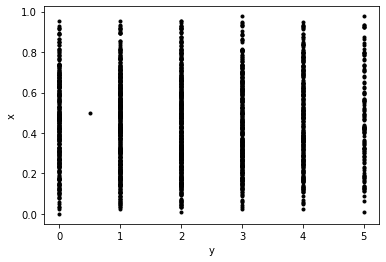
\includegraphics[width=0.3\textwidth]{Post_4_betabinom1}}
\subfloat[][Distributions]{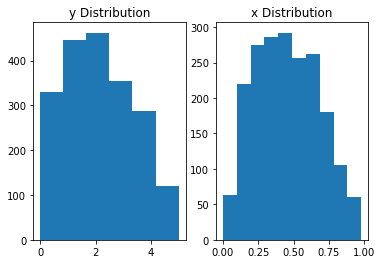
\includegraphics[width=0.3\textwidth]{Post_4_betabinom2}}
\caption{Gibbs Sample of Dependent Distribution Broken into Marginals}
\end{figure}

\vspace{5mm}

The obvious question to ask is how generalizable is the Gibbs Sampling method? The answer is that only parameters that are independent or have known/simple marginal distributions with all other parameters can be sampled using this method. Therefore, simple statistical models such as those with normal distributions are often sampled this way, but for many practical problem we need something more...powerful.

\section{Hamiltonian-Monte Carlo Sampling}

A more robust way of sampling distributions is via a Hamiltonian-Monte Carlo (HMC) sampling method where we (1) propose a new sample $\theta_p$ then (2) use the posterior $Pr(\theta | x)$ to determine if that, in fact, is representative of a sample of the underlying posterior. We write $Pr(\theta | x)=p(\theta)$ for simplicity.

\vspace{5mm}

\begin{algorithm}[H]
 \KwData{$p(\theta)$ Posterior Equations}
 \KwResult{$\Theta \sim Pr(\theta)$ Posterior Sample}
Initialize $\theta$\;
\For{$k = 1:K$ Samples}{
$\theta_p \sim p(\theta,C)$\;
$p(\theta) = p(\theta)$\;
$p(\theta_p) = p(\theta_p)$\;
$q(\theta |\theta_p) = p(\theta | \mu=\theta_p, C)$\;
$q(\theta_p | \theta) = p(\theta_p | \mu=\theta, C)$\;
$\alpha = min\{1,\dfrac{p(\theta_p) q(\theta | \theta_p)}{p(\theta) q(\theta_p | \theta)}\}$\;
$Pr(\theta = \theta_p = \Theta_k) = \alpha$\;}
 \caption{Hamiltonian-Monte Carlo Sample}
\end{algorithm}

\vspace{5mm}

After sampling these distributions we accept $\theta = \theta_p$ with probability $\alpha$ (using a random uniform number generation scheme for example). In Algorithm 2 note that in addition to the posterior $p(\theta)$ we have a proposal distribution $q(\mu,C)$ which is centered at some $\mu$ with multivariate variance $C$. For the most part:

\begin{align*}
q(\mu,C) = N(\theta,I)
\end{align*}

Or to make the sampler be more conservative:

\begin{align*}
q(\mu,C) = N(\theta,\sigma I) \;, \sigma < 1
\end{align*}

\vspace{5mm}

So we are likely to accept a $\theta_p$ if $p(\theta_p)>p(\theta)$ (improvement in posterior).

\vspace{5mm}

Let's take an example of two normal distributions and, because I'm bad at statistics and don't want to integrate out the marginals, will solve it with the HMC algorithm.

\begin{align*}
p(\theta_0,\theta_1,\Sigma = \begin{pmatrix} 1 & 0.2 \\ 0.2 & 1 \end{pmatrix})
\end{align*}

\begin{figure}[h]
\centering
\subfloat[][Sample]{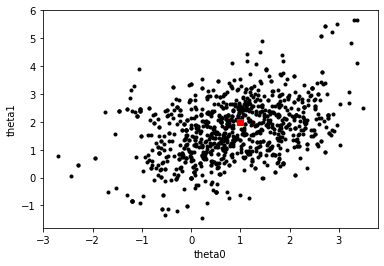
\includegraphics[width=0.3\textwidth]{Post_4_hmc1}}
\subfloat[][Distributions]{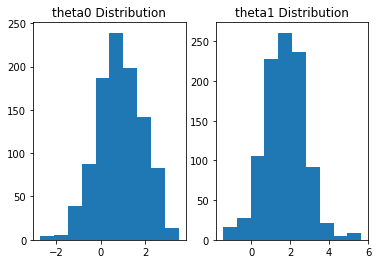
\includegraphics[width=0.3\textwidth]{Post_4_hmc2}}
\subfloat[][Chains]{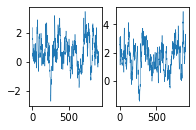
\includegraphics[width=0.3\textwidth]{Post_4_hmc3}}
\caption{Hamiltonian-Monte Carlo Sample of Correlated Normal Distributions}
\end{figure}

\vspace{5mm}

From Figure 4 we have the expected correlated sample and distributions of means. I have added the chains (a plot of the matrix $\Theta$) of the HMC sample in Figure 4(c) because oftentimes difficult to solve posteriors require analysis of the chains of $\Theta$. The important thing to understand from this is that it was very easy to put together the HMC algorithm (even if it looks longer and more confusing) because I only had to write out a single posterior rather than have a bunch of marginals. As long as the model in question has a tractable posterior distribution it can be integrated using HMC, and because of Bayes Rule mentioned in the beginning of this post, posteriors can just take the form of products of any distribution!

\vspace{5mm}

Next week we will be talking about more MCMC and Bayesian Modeling with some more examples!

\end{document}